\section{Función de validación}
\markright{FUNCIÓN DE VALIDACIÓN}
Igual que en búsqueda lineal podíamos agregar funciones más complicadas a la hora de buscar la respuesta, lo mismo sucede en búsqueda binaria. A veces requeriremos de más código que una simple comparación para saber en cual mitad esta la respuesta.

Veamos unos ejemplos.


\subsection*{Ejemplo: Bicicleta de Karel II}
Karel ha comprado una bicicleta eléctrica con la que planea completar un recorrido. El recorrido se puede ver como \(N\) colinas en línea recta tal que la \(i\)-ésima colina tiene altura \(h_i\). Karel comienza en la colina hasta la izquierda y quiere terminar en la ultima colina de hasta la derecha.

Cuando Karel sube un metro gasta \(1\) unidad de energía, mientras que bajar un metro recupera \(1\) unidad de altura. Si Karel en algún momento necesita subir, pero su batería tiene 0 de energía, Karel se quedará atorado y no terminará el recorrido.

Por suerte al inicio hay una estación de recarga donde Karel puede recargar su bicicleta. Como nota, la batería tiene capacidad \(R\) y jamás podrá almacena más energía que \(R\).

Actualmente Karel tiene \(0\) de energía, Determina cuál es la menor cantidad de energía que es necesaria recargar al inicio para completar el recorrido. O determina si es imposible hacer el recorrido con la bicicleta de Karel.

\subsubsection*{Entrada}
La primera línea tiene dos enteros, el valor de \(N\) y \(R\).

En la siguiente línea vienen \(N\), enteros separados por espacios, siendo la altura de las colinas de izquierda a derecha. Recuerda que Karel comienza en la primera colina y quiera terminar en la última.
\subsubsection*{Salida}
Un entero, representando la menor cantidad de energía necesaria para completar el recorrido. Si Karel no puede completar el recorrido, imprime \(-1\).

\subsubsection*{Casos ejemplo}
\begin{casebox3}	
	\ecase{
		6 8\\
		4 6 3 5 7 
	}
	{3}
	{
		Karel inicia con 3 de energía, moverse de   \\
		la primera a la segunda colina le toma 2,  \\
		ahora tiene 1.\\
		Luego avanza y se recarga 3,\\
		ahora tiene 4.\\
		Después continua y se consume 2, ahora tiene 2. \\
		Vuelve a avanzar quedándose con 0 de energía. \\		
		Pero luego avanza y se recarga a 5. \\
		Finalmente avanza para termina con 5. \\
	}
	\ecase{
		5 6\\
		1 10 1 2 0
	}
	{-1}
	{}
	\hline
\end{casebox3}	

\subsubsection*{Límites}
\begin{plimits}
	\item \(2\leq N, R \leq 10^5\)
	\item \(0\leq h_i\leq 10^9\)
\end{plimits}

Fuente: OMIS online 2022.\\
\footnotesize{(\omegauplink{Bicicleta-de-Karel})}

\subsection*{Solución}
Este problema 1.6 de búsqueda lineal con validación en la página \pageref{bicicleta}, si no sabes resolverlo con búsqueda lineal para los límites de allí, primero descubre esa solución.

Esta vez, los límites son más estrictos, de forma que la solución estándar con búsqueda lineal no funciona, pero veamos cual es porque nos será útil.
\\

La respuesta siempre estará entre \(0\)  y\(R\). La búsqueda lineal funciona de la siguiente manera.
\begin{lstlisting}
	int respuesta=-1;
	for (int e=0; e<=R; e++) {
		if (funciona(e)) {
			respuesta=e;
			break;
		}
	}
\end{lstlisting}

Y la función \verb|bool funciona(int e)| te regresa verdadero si Karel puede completar el recorrido comenzando con \(e\) de energía.

Esta función simplemente simula el recorrido para ver si Karel se atora en algún momento. Se ve de la siguiente forma:

\begin{lstlisting}
	bool funciona(int e) {
		for (int i = 1; i <N; i++){
			e-=A[i]-A[i-1];
			if (e > R) 
			e=R; //Limita la energia
			if (e < 0)
			return false;			
		}
		return true;
	}
\end{lstlisting}

La función \verb|funciona()| tiene una complejidad de \(O(N)\) y como es llamada en \(R\) valores, la complejidad total es \(O(RN)\).

Pero ahora veamos dos hechos importantes:
\begin{itemize}
	\item Si funciona(m) cumple, también lo hará cualquier valor mayor que \(m\).
	\item Si funciona(m) falla, también lo hará cualquier valor menor que \(m\).
\end{itemize}

Es decir, el rango de búsqueda se ve de la siguiente forma:

\begin{center}
	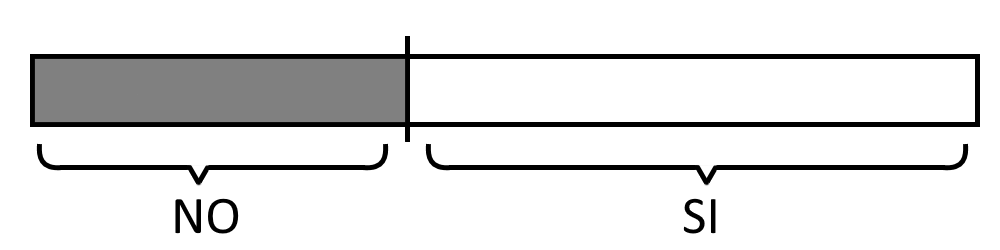
\includegraphics[scale=0.3]{binprop}
\end{center}

Esto hace que podamos hacer búsqueda binaria para encontrar el primer SI.

El código se verá como:

\begin{lstlisting}
	int a=0,b=R;
	while(a!=b) {
		int m=(a+b)/2;
		if (funciona(m)) {
			b=m;
		} else {
			a=m+1;
		}
	}
	int respuesta=-1;
	if (funciona(a))
	respuesta=a;
\end{lstlisting}

\section{Complejidad}

La complejidad de la búsqueda binaria es entonces \(O(logN)\), donde \(N\) es el tamaño del espacio de búsqueda porque \(logN\) nos dice cuantas veces \(N\) puede ser dividido entre dos. 

Pero también, en cada paso de la búsqueda podemos usar una llamada de validación. En el ejemplo anterior estamos llamando a \verb|funciona()| que tiene complejidad \(O(N)\), por lo tanto, la complejidad total es \(O(NlogR)\).

Es decir, la complejidad de una búsqueda binaria es \(O(busqueda \times validacion)\) que es igual a \(O(logN \times validacion)\).


\section*{Problemas de práctica}
\addcontentsline{toc}{section}{Problemas de práctica}

\begin{exercise}
	\problema[barcos-turisticos]{Barcos turísticos}{\omegauplink{Barcos-turisticos}}
\end{exercise}

\begin{exercise}
	\problema{Subcadena de suma K}{TODO}
\end{exercise}